% syllabus.tex  written 8.16.06
% author: cameron hummels
% syllabus for Earth, Moon \& Planets Fall 2006
\documentclass[letterpaper,11pt]{article}
\usepackage{epsfig}
\textwidth=6.5in
\textheight=9.6in
\topmargin=-0.75in
\oddsidemargin=0.0in
\evensidemargin=0.0in

\pagestyle{empty}

\begin{document}
\begin{center}
\textbf{\LARGE{Lab 8 -- Convection (it's Everywhere!)}}

\end{center}
\vspace{.2in}

\begin{center}
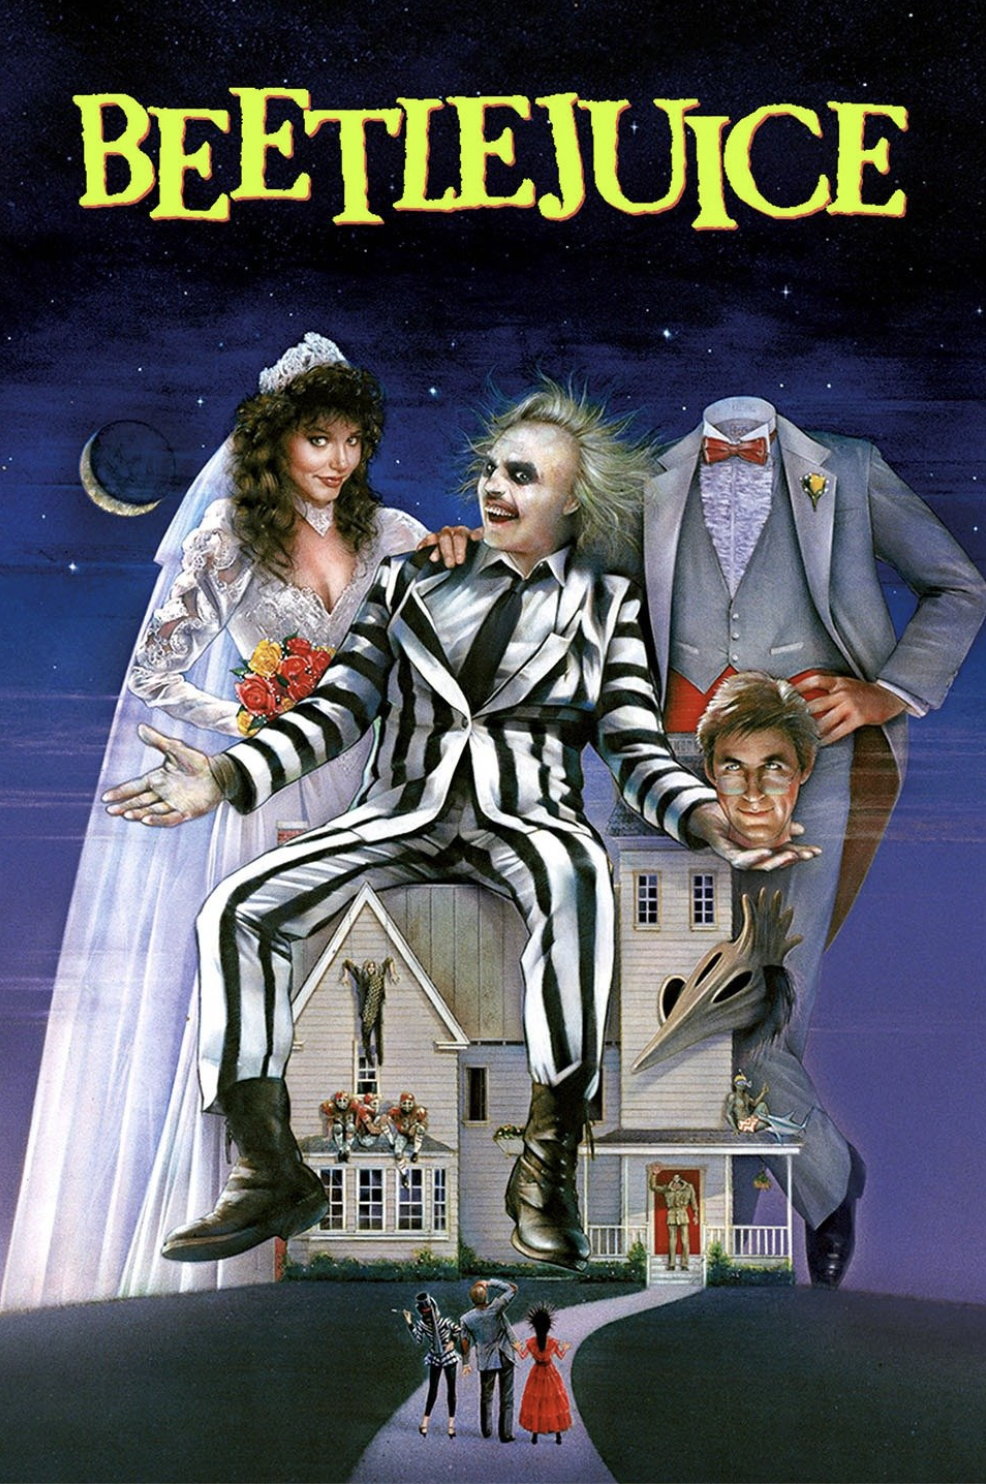
\includegraphics[width=4cm]{movie.png}
\vspace{.1in}
\end{center}

Convection is a powerful process, both in our day-to-day lives and in distant stars (including our Sun). Today we will learn about convection from the largest scales down to the smallest. You will learn about the mysterious star Betelgeuse and how convection can explain its unusual behavior. You will use your intuition, along with a helpful simulation, to think about convection on Earth. In addition, you will do an in-class experiment to investigate further. 
\vspace{.2in}

\textbf{\Large{Thinking about Convection in Stars}}
\vspace{.2in}

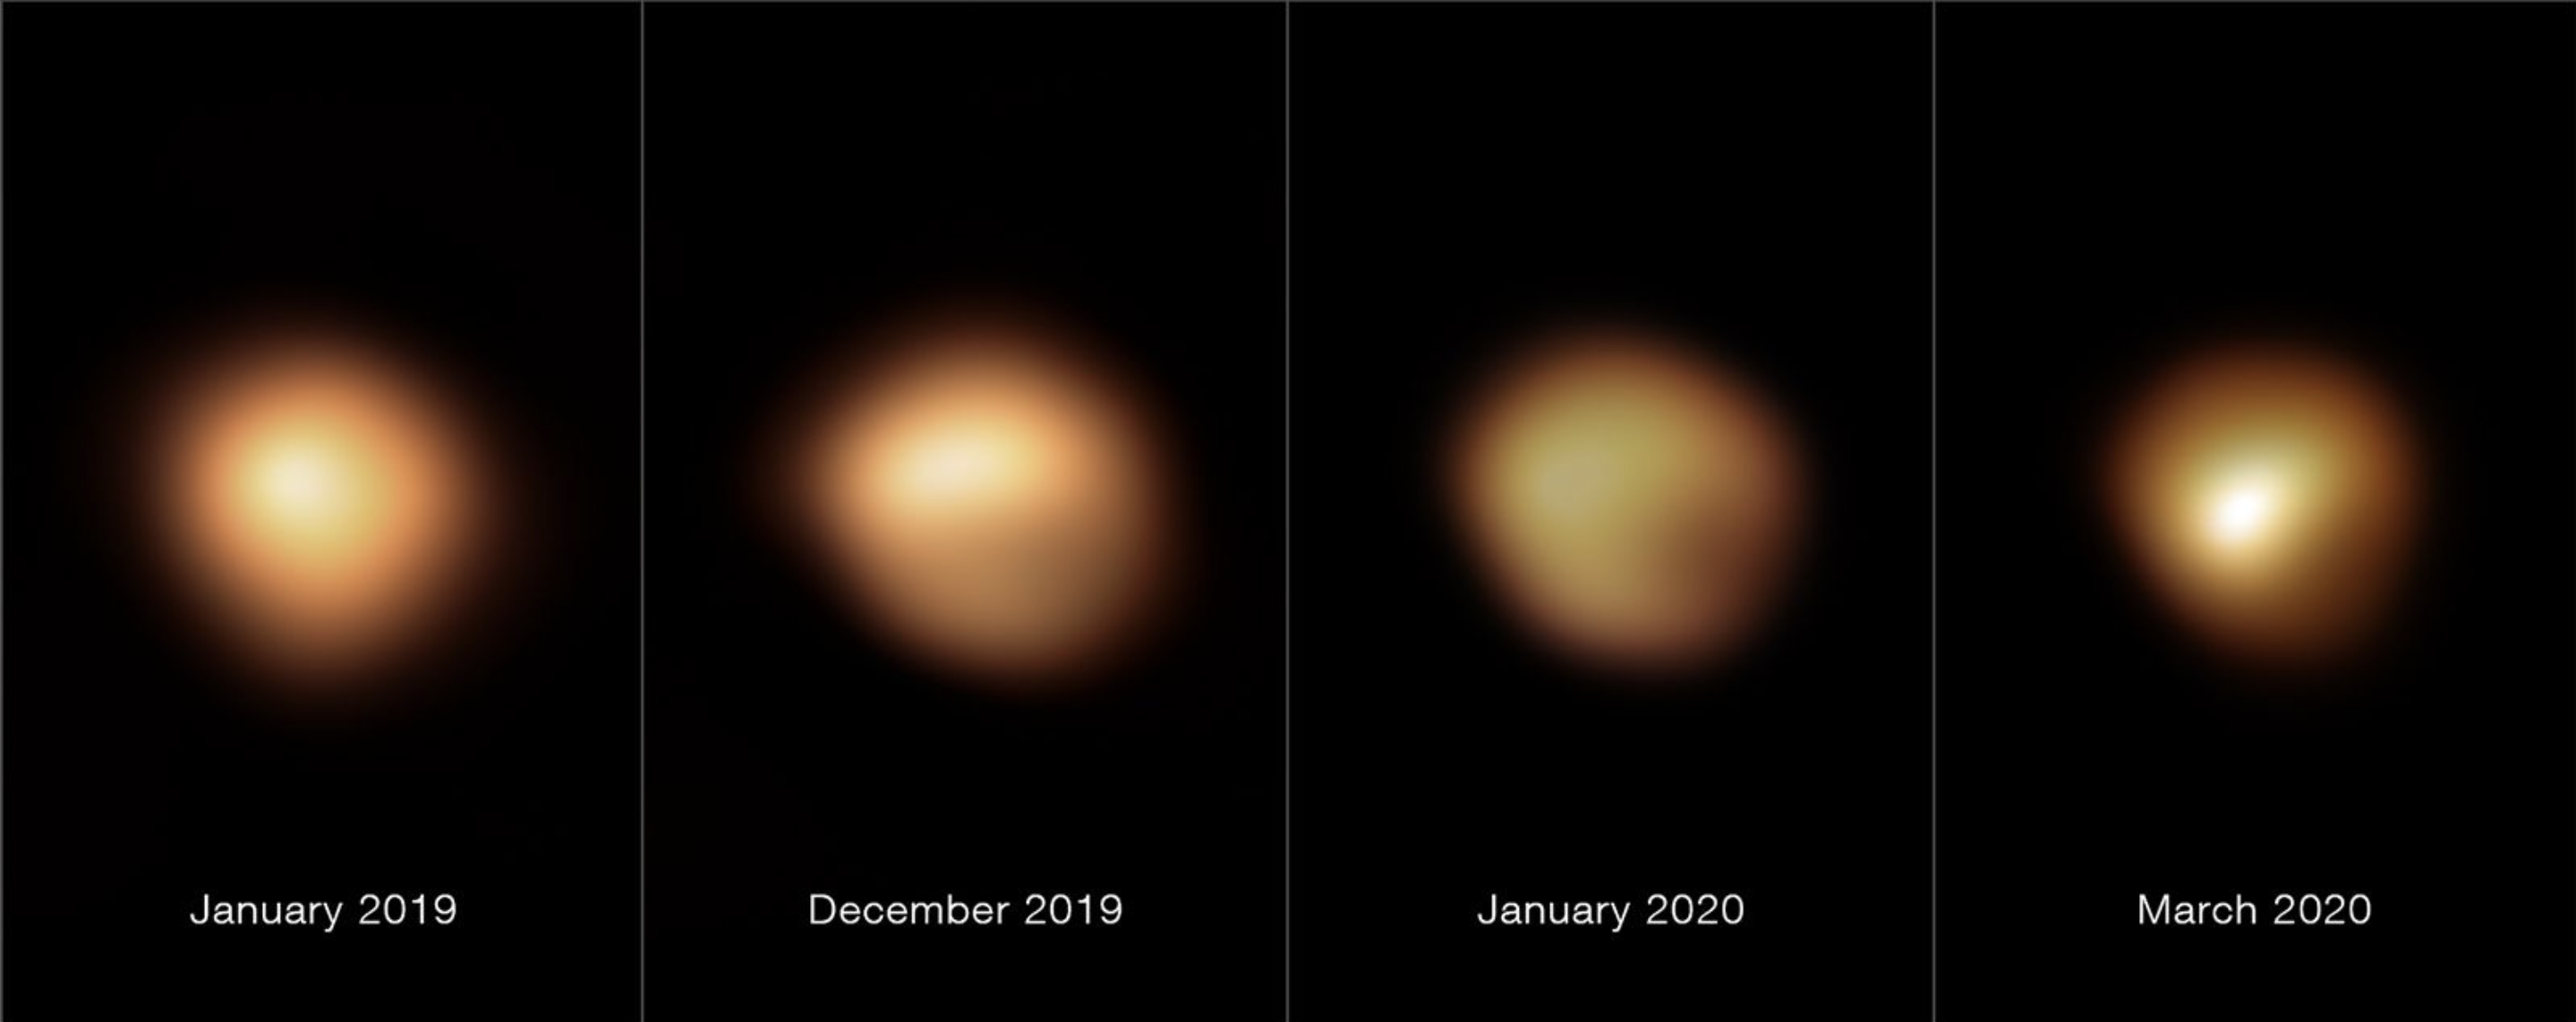
\includegraphics[width=\textwidth]{dimming.png}
\vspace{.1in}

We may be a couple days past Halloween, but we can stick kick-off class by thinking about a rather mysterious star. We will watch this video, by Columbia Astronomy Professor David Kipping, called ``Betelgeuse Explained": https://www.youtube.com/watch?v=5bvuwTuGnkc \\

After watching the video, answer the following questions in your research notebook: 

\vspace{.1in}
\begin{enumerate}
\item What is so strange about the star Betelgeuse?
\item What are some ways it is different than our Sun?
\item What are possibilities for Betelgeuse's death? Do we think it will go supernova anytime soon, why or why not?
\item What are the two theories that explain Betelgeuse's dimming? Which do you think seems most plausible (please explain -- there is no right answer). 
\item Where can we see convection on Betelgeuse (and on our own Sun)? What can we learn about the size of the convection cells?
\vspace{.2in}

\textbf{\Large{Thinking about Convection on the Earth}}
\vspace{.1in}

Take five minutes or so to play with this simulations: https://javalab.org/en/convection_en/ \\

Imagine each dot is a gas or water particle. You can move the location of the burner (as well as turn it on or off by checking or un-checking a box) to heat the particles. Check the ``time-lapse'' box to see the particles' ``tracks'' as they experience heating. 

\item Now, imagine if instead of gas or water, these are plasma particles (like what would be found on the surfaces of stars). If I looked at the box of particles from a top-down view after turning on the burner, what would I see that reminds me of the surface of the Sun or Betelgeuse?

\item Is cold water or hot water more dense?  How about cold or hot air? How do you know?
\item Would a blob of a cold fluid rise or sink if it were surrounded by 
hot fluid?  What about the inverse situation?
\item What parts of the Earth receive the most sunlight (per unit area)?
What parts receive the least sunlight? (Hint: Think about where the climate is hottest/coldest)
\item Sketch a cross-section of the Earth and its atmosphere and indicate
(with arrows) where you think air currents might rise and where they might
sink.
\item Surface winds blow from areas of sinking air (high pressure) to 
areas of rising air (low pressure).  High-altitude winds blow from areas
of rising air to areas of sinking air.  Explain why winds blow this way.
Draw the surface winds on your diagram.
\vspace{.2in}

\textbf{\Large{Visualizing Convection}}
\vspace{.1in}

Now, let's do some in-class experiments to solidify our understanding of convection!
\vspace{.1in}

\textbf{Materials}
\begin{itemize}
\item Hot or warm water
\item Clear cup
\item Paprika or some other visibly ground spice
\item Food Coloring
\item Ice Cube
\end{itemize}

\vspace{.1in}
\textbf{Procedure}
\vspace{.1in}

Fill a cup most of the way with hot water.  Let it stand for 2-3 minutes to get
rid of currents.  Sprinkle spice in the water.  Gently put ice cube in cup.
Now put a single drop of food coloring on ice cube.  Observe the movement of 
the water using your tracers (color and spice).

\vspace{.1in}
\textbf{Analysis}
\vspace{.1in}

\item Draw and describe how the water moves.  Where does it move fastest?
\item Why does it behave this way?  Explain.
\vspace{.5in}

\textbf{\Large{Relative Densities of Fresh and Salt Water}}

\vspace{.1in}
\textbf{Materials}
\vspace{.1in}

\begin{itemize}
\item Fine table salt
\item Water
\item Clear Cup
\item Food coloring or spice
\item spoon
\end{itemize}

\vspace{.1in}
\textbf{Procedure}
\vspace{.1in}

With your lab group, come up with a method for determining whether fresh 
or salt water is more dense.  Feel free to refine or change your methods 
as you go along.  Record your procedure and observations.

\vspace{.1in}
\textbf{Analysis}
\vspace{.1in}

\item Is salt water or fresh water more dense?
\item Would a blob of salt water rise or sink if it were surrounded by fresh water?  Vice versa?
\item Can you tell what would happen to a blob of warm salty water surrounded by cold fresh water?
\item Is a layer of fresh water on top of salt water stable?  Is a layer of salt water on top of fresh water stable?
\vspace{.1in}

\textbf{\Large{Convection inhibited by a density gradient}}

\vspace{.1in}
\textbf{Materials}
\vspace{.1in}

\begin{itemize}
\item fine table salt
\item warm/hot water
\item clear cups
\item food coloring or spice
\item ice cubes
\item spoon
\end{itemize}

\vspace{.1in}
\textbf{Procedure}
\vspace{.1in}

Put  heaping spoonfuls of salt in a beaker and add water up to near the top.  Mix well.  Pour 2/3rds into one cup, pour the other 1/3rd into the other cup.  Let the cups sit undisturbed until the brine has stopped swirling.

Put 1/3rd of a cup of fresh water into a clean cup.  In the cup with the smaller amount of brine, hold a spoon horizontally and lower it into the cup until it rests on the surface of the brine.  Put the tip of the spoon against the side of the cup.  Now very slowly and steadily pour the fresh water into the spoon to minimize the mixing between the fresh and salt water.  If you have done it right there should be a clearly-visible layer of fresh water on the salt water.  This step is crucial.  Let the cup sit for 2-3 more minutes.

Make sure you have two ice cubes handy, then put a single drop of food coloring in each cup.  Do NOT stir. 
\item Do you observe any differences between what happens to the drop in each cup?

\vspace{.1in}

Now gently set and ice cube in each cup right on top of the spot of food coloring.  
\item Observe the cups for several minutes (until most of the ice is melted) and record any differences between what happens in the two cups.  Also note any changes that occur over time.

Once most of the ice is melted in both cups, give each cup one gentle stir with a spoon handle touching the bottom of the cup.
\vspace{.1in}
\item Record any differences between what happens in each cup.

\item Explain any differences you observed between the two cups.
\item Explain any differences between what happened in this experiment and what happened in the ``visualizing convection'' activity.
\item Explain any changes that occurred as the ice cubes melted.

\vspace{.1in}
\textbf{Other examples of Convection in Earth's Seas}
\vspace{.1in}

The Dead Sea used to be stable against convection because the deep layers of the lake are saturated with salt, while the surface layers were replenished with fresh water from the Jordan and other rivers.  This kept the surface water from sinking to the bottom even if it was colder than the underlying layers. As people started to use more and more river water for irrigation, less fresh water was reaching the Dead Sea.  In the winter of 1978-1979, the Dead Sea turned over, bringing salt-saturated water from the depths up to the surface.  

% \item Why was the surface stable against convection, despite being colder than
% the underlying layers?

% As people started to use more and more river water for irrigation, less fresh water was reaching the Dead Sea.  In the winter of 1978-1979, the Dead Sea turned over, bringing salt-saturated water from the depths up to the surface.  

% \item Why did this happen in the winter?

% \vspace{.1in}
% \textbf{The Ocean Conveyor}
% \vspace{.1in}

The Gulf Stream and the North Atlantic Current are important ocean currents that transport heat from the equator to the waters around Europe as part of the Ocean Conveyor.  In the tropics, intense sunlight warms the surface waters of the ocean and causes rapid evaporation that increases its salinity. The Gulf Stream carries this warm salty water along the East Coast of North America, then the North Atlantic Current carries it North-Eastward into the waters off Europe.  When the current reaches the North Atlantic, it begins to cool off and then sinks and forms a river that returns South through the depths of the ocean.

% \item Why would the water from the tropics sink when it reaches the same temperature as the surrounding water (or even before)?

If anything disrupted the Ocean Conveyor, preventing it from transporting equatorial heat to the North, average air temperatures could drop by as much as 5 degrees Kelvin around the North Atlantic, and Europe, in particular, could have much harsher winters.

% As the polar ice cap and arctic glaciers melt, they add fresh water to the surface of the North Atlantic.  

% \item Can you think of a reason why the Ocean Conveyor might be slowed or disrupted if this water dilutes the water from the tropics?  What about if the fresh water forms a cap over the North Atlantic?
% \vspace{.1in}
% \vspace{.1in}

\vspace{.3in}
\textbf{Reflections}
\vspace{.1in}

\noindent In your lab notebook, write a brief (2-4 sentences) reflection on what you took away from this lab. If you need some inspiration, what was your favorite exercise and why? Alternatively/in addition, describe something new you learned.


\end{enumerate}

\end{document}